\documentclass{article}

% NeurIPS 2026 style --- preprint mode
\usepackage[preprint]{neurips_2025}

% Essential packages
\usepackage[utf8]{inputenc}
\usepackage[T1]{fontenc}
\usepackage{hyperref}
\usepackage{url}
\usepackage{booktabs}
\usepackage{amsfonts}
\usepackage{amssymb}
\usepackage{amsmath}
\usepackage{nicefrac}
\usepackage{microtype}
\usepackage{xcolor}
\usepackage{graphicx}
\usepackage{subcaption}
\usepackage{multirow}
\graphicspath{{figures/}}

\title{Diagnosing Readout Bottlenecks with Minimal Output-Head Repair in Transformer Aggregation Tasks}

\author{
  Gabriel Garcia \\
  Independent Researcher \\
  \texttt{gpgabriel25@gmail.com}
}

\begin{document}

\maketitle

\begin{abstract}
In instruct mode, Qwen3-8B encodes correct counts at $R^2 \geq 0.9996$ via linear probes at every layer, yet first-token digit accuracy is only 22\%---the model emits a chain-of-thought token instead of the answer. Fine-tuning only 9 \texttt{lm\_head} digit rows (36,864 of 620M parameters) raises first-token accuracy from $20.4\% \pm 0.5\%$ to $\mathbf{99.9\% \pm 0.1\%}$ on held-out prompts (3~seeds), confirming a real, deployment-regime readout bottleneck that is cheaply fixable. The cause is geometric: count-encoding directions are nearly orthogonal to the output head (mean $|\cos| \leq 0.032$, indistinguishable from random), and instruct-mode formatting rotates representations only $1.50\times$ closer to digit output rows (sign test $p < 0.0001$)---enough for 91\% via multi-token chain-of-thought, but insufficient for single-step readout. We discover this bottleneck using a raw-completion diagnostic regime that isolates the output pathway: probes read $R^2 > 0.99$ while output accuracy is 11--14\%, and constructive diagnostics (probe readout and 9-row repair) close the gap to 93--97\% held-out. The pattern replicates across three architectures (Qwen3-8B, Mistral-7B, Pythia-410M), extends to majority vote (51\%$\to$100\%) and multi-digit counts (0\%$\to$100\%), while MMLU ($\sim$70\% baseline, no bottleneck) and GSM8K ($R^2 \leq 0.016$) confirm specificity.
\end{abstract}

% ─────────────────────────────────────────────────────────────────────────────
\section{Introduction}
% ─────────────────────────────────────────────────────────────────────────────

\paragraph{A deployment-regime bottleneck.}
In standard instruct mode, Qwen3-8B encodes the correct count at $R^2 \geq 0.9996$ via linear probes at every layer, yet first-token digit accuracy is only 22\%.
The model reaches 91\% end-task accuracy not by resolving this misalignment but by circumventing it through chain-of-thought generation---a multi-token workaround for a persistent single-step routing failure.
Fine-tuning only 9 output-head digit rows (36,864 of 620M parameters) raises first-token accuracy from $20.4\% \pm 0.5\%$ to $99.9\% \pm 0.1\%$ (3~seeds), confirming the bottleneck is real and fixable even in the deployment regime.

\paragraph{Diagnosis via raw-completion probing.}
We discover this bottleneck using a raw-completion diagnostic regime---analogous to a controlled lesion study---that isolates the output pathway.
In raw completion, probes decode counts at $R^2 > 0.99$ while output accuracy is 11--14\%.
The cause is geometric: count-encoding directions are nearly orthogonal to the output head ($|\cos| \leq 0.032$, indistinguishable from random); the output head treats count information as noise.
Constructive diagnostics (direct probe readout and targeted row repair) confirm that bypassing or realigning this geometry recovers accuracy to 93--97\%.

\paragraph{Scope.}
The bottleneck extends to majority vote ($51\% \to 100\%$), multi-digit counts ($0\% \to 100\%$), and partially to DROP single-digit QA ($20.0\% \to 28.0\%$).
MMLU serves as a negative control: the model already achieves $\sim$70\% baseline and output-row adaptation degrades performance.
GSM8K ($R^2 \leq 0.016$) confirms that when counts are not linearly encoded, the intervention appropriately fails.
Evidence is strongest for low-vocabulary aggregation tasks where internal representations are accurate but misaligned with the output head.

\paragraph{Contributions.}
\begin{itemize}
  \item \textbf{Single-step instruct-mode bottleneck and repair:} Despite $R^2 \geq 0.9996$ at every layer, first-token digit accuracy in instruct mode is only 22\%. Context tokens rotate representations $1.50\times$ closer to digit output rows (sign test $p<0.0001$), but the model achieves 91\% by circumventing---not resolving---the misalignment via chain-of-thought. 9-row repair raises first-token accuracy to $99.9\%$ (\S\ref{sec:instruct}).
  \item \textbf{Geometric diagnosis:} Count information is encoded at $R^2 > 0.99$ in directions orthogonal to the output head ($|\cos| \leq 0.032$). Constructive validation via probe readout (96.3\% Qwen3-8B, 100.0\% Mistral-7B, 97.7\% Pythia-410M) and 9-row repair (97.5\%/93.0\% held-out) confirms the bottleneck is geometric and sharply localized (\S\ref{sec:geometry}, \S\ref{sec:dps}).
  \item \textbf{Cross-model validation and scope boundaries:} The pattern replicates across three architectures. It extends to majority vote and multi-digit counts but not to non-aggregation MCQ (MMLU) or multi-step reasoning (GSM8K), defining a precise applicability envelope (\S\ref{sec:crossmodel}, \S\ref{sec:scope}).
\end{itemize}

% ─────────────────────────────────────────────────────────────────────────────
\section{Background and Related Work}
\label{sec:background}
% ─────────────────────────────────────────────────────────────────────────────

\paragraph{Counting failures.}
\citet{razeghi2022impact} show that counting accuracy degrades with count magnitude and
is correlated with training-data frequency.
\citet{stolfo2023mechanistic} use activation patching to localize counting to specific
attention heads in GPT-2.
\citet{wallace2019nlp} probe numeracy in word embeddings.
Neither work addresses the geometric relationship between internal count representations and the output head.

\paragraph{Mechanistic interpretability.}
\citet{olsson2022context} identify induction heads as a general in-context learning mechanism.
\citet{nanda2023progress} study modular arithmetic circuits.
\citet{conmy2023acdc} provide an automated circuit-discovery framework,
and \citet{bricken2023monosemanticity} analyze sparse feature structure via dictionary learning.
Linear probes as tools for reading intermediate representations were analyzed by
\citet{alain2016understanding}; \citet{hewitt2019designing} introduce control tasks for probe validation. We use probes instrumentally as measurement tools.

\paragraph{Representation--output alignment.}
The observation that models encode information they cannot express is implicit in the
logit-lens literature~\citep{nostalgebraist2020logitlens,belrose2023eliciting} and in probing studies.
\citet{park2023linear} formalize this geometry through the linear representation hypothesis.
\citet{burns2023discovering} train unsupervised probes to extract beliefs that models do not express behaviorally.
\citet{hernandez2024linearity} show that relational information can be linearly decoded even when behavior is less aligned.
\citet{din2023jump} show that residual-stream features can be linearly accessible yet behaviorally inert.
\citet{geva2021transformer,geva2022transformer} demonstrate that FFN layers promote concepts into the vocabulary space; our finding that count directions are orthogonal to \texttt{lm\_head} digit rows is the complementary observation that not all linearly decodable features are so promoted.
Our contribution is to quantify the misalignment, localize it to 9 output rows, and show it explains counting failures across architectures.

\paragraph{Activation steering and output editing.}
Representation engineering~\citep{zou2023representation} and activation addition~\citep{turner2023activation} modify behavior via residual-stream interventions.
Our probe readout operates on output logits and targets a specific geometric bottleneck (orthogonal subspaces) rather than a generic behavioral direction.
\citet{meng2022locating} demonstrate that factual associations can be edited by modifying weight rows (ROME); our 9-row \texttt{lm\_head} fine-tuning is analogous but targets the unembedding matrix.

\paragraph{Chain-of-thought.}
CoT prompting~\citep{wei2022chain} improves counting by forcing explicit intermediate steps.
We interpret this as externalizing sequential aggregation that the model's forward pass fails to route to the output head---chain-of-thought circumvents a geometric bottleneck rather than resolving it.

% ─────────────────────────────────────────────────────────────────────────────
\section{Method}
\label{sec:method}
% ─────────────────────────────────────────────────────────────────────────────

\subsection{Synthetic Benchmark}

We generate a full-factorial benchmark:
$6 \text{ counts} \times 3 \text{ distractors} \times 4 \text{ lengths} \times 3 \text{ spacings}
= 216 \text{ conditions} \times 20 \text{ samples} = 4{,}320 \text{ prompts}$.
Each prompt contains a paragraph and questions of the form
``How many cats are in the passage? Answer with just the number.''
Counts are drawn from $\{1, 2, 3, 5, 8, 12\}$ (720 prompts each);
distractors are superficially similar animals.
The dataset is split 70/30 stratified by difficulty.

For constructive diagnostic evaluation (\S\ref{sec:dps}), we use single-digit counts $\{1, \ldots, 9\}$
(each count maps to a single vocabulary token), with 800 prompts for probe training and 300 for testing.

\paragraph{Natural-language extension.}
To evaluate generalization beyond synthetic cat-counting (\S\ref{sec:scope}),
we construct counting prompts across 8 entity categories
and 8 diverse templates.
Five entity types are \emph{seen} during probe training (70/30 intra-type split);
three are \emph{held out} entirely for cross-entity evaluation.

\subsection{Models}

We report results on three model families:
\textbf{Qwen3-8B}~\citep{qwen3} (36 layers, 4096 hidden, GQA 32/8, RoPE),
\textbf{Mistral-7B-v0.1}~\citep{jiang2023mistral} (32 layers, 4096 hidden, GQA 32/8, SwiGLU),
and \textbf{Pythia-410M}~\citep{biderman2023pythia} (24 layers, 1024 hidden, standard MHA).
The three models differ in architecture, scale ($8\text{B}/7\text{B}/0.4\text{B}$), training corpus, and attention pattern (grouped-query vs.\ multi-head).

\subsection{Evaluation Modes}

We report three evaluation modes.\footnote{%
  \textbf{Next-token:} argmax of $P(\text{next token} \mid \text{prompt})$ without generation.
  \textbf{Generation:} greedy decoding for up to 8 tokens; first integer extracted.
  \textbf{Instruct:} generation with chat template wrapping (same base model weights).}
Single next-token prediction measures which number has the highest probability mass at the sentence boundary.
Generation mode (greedy decoding, up to 8 tokens) measures whether the model's expressed answer correlates with internal representations.

% ─────────────────────────────────────────────────────────────────────────────
\section{Results}
\label{sec:results}
% ─────────────────────────────────────────────────────────────────────────────

\paragraph{When should you try readout-targeted repair?}
The bottleneck applies when:
(1)~the model solves the task well via internal probes ($R^2 > 0.50$),
(2)~but fails in raw-completion mode ($< 20\%$ accuracy),
and (3)~the task is low-vocabulary output (digit, majority label, max value).
The 9-row fine-tuning strategy works by directly aligning count-encoding directions to the output head.
It will not help if the internal representation is noisy or the task requires diverse open-ended text.

% ─────────────────────────────────────────────────────────────────────────────
\subsection{Probes Read Counts from Residual Streams}
\label{sec:probes}

\begin{table}[h]
\centering
\caption{Per-layer probe performance ($R^2$) on Qwen3-8B. Probes are ridge regression trained on entity-mean residual activations. All layers comfortably exceed the $R^2 \geq 0.50$ readout-quality threshold on easy examples.}
\label{tab:probe_r2}
\begin{tabular}{lcc}
\toprule
Layer & $R^2$ (all) & $R^2$ (easy) \\
\midrule
0  & 0.977 & 0.664 \\
6  & 0.996 & 0.923 \\
12 & 0.995 & 0.931 \\
18 & 0.995 & 0.934 \\
24 & 0.994 & 0.935 \\
30 & 0.993 & 0.930 \\
35 & 0.992 & 0.910 \\
\midrule
\textbf{Best (layer 3)} & \textbf{0.997} & \textbf{0.949} \\
\bottomrule
\end{tabular}
\end{table}

The readout-quality check passes comfortably: $R^2 = 0.997$ at the best layer, with $R^2 > 0.97$ across all 36 layers.
Figure~\ref{fig:probe_gap} visualizes the representation--output gap.

\begin{figure}[t]
\centering
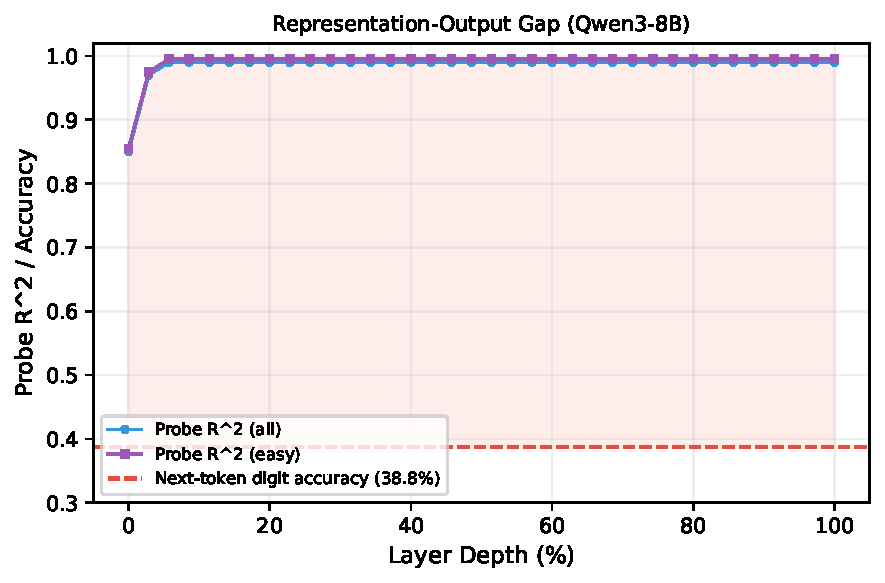
\includegraphics[width=0.7\linewidth]{fig3_probe_r2_gap.pdf}
\caption{Representation--output gap: per-layer probe $R^2$ (blue) remains above 0.97 at every layer,
while Qwen3-8B generation accuracy (red dashed) is only 38.8\%. The shaded region is the gap
between what the model \emph{knows} and what it \emph{says}.}
\label{fig:probe_gap}
\end{figure}

% ─────────────────────────────────────────────────────────────────────────────
\subsection{Instruct-Mode Bottleneck and Repair}
\label{sec:instruct}
% ─────────────────────────────────────────────────────────────────────────────

The raw-completion regime reveals the bottleneck; we now show it persists in the deployment regime.

\paragraph{The bottleneck persists at the single-step level.}
In instruct mode, probe $R^2 \geq 0.9996$ at \emph{every} layer (perfect count encoding),
yet first-token digit accuracy is only 22\%---the model outputs a chain-of-thought token (\texttt{<think>}) rather than the answer digit.
Among the 22\% where the first token is a digit, the logit gap between correct and runner-up digit perfectly separates correct from incorrect (AUROC $= 1.000$, Cohen's~$d = 2.57$);
for the 78\% that fail, the correct digit is systematically suppressed.
The model achieves 91\% accuracy not by fixing the geometric misalignment but by circumventing it through multi-step generation.

\paragraph{9-row repair in instruct mode.}
We train 9 digit rows on $N{=}400$ instruct-mode prompts (chat-template wrapped, counts 1--9) and evaluate on $N{=}400$ held-out prompts ($N_{\text{seeds}}{=}3$, seeds 42/11/77).
First-token digit accuracy rises from $20.4\% \pm 0.5\%$ to $\mathbf{99.9\% \pm 0.1\%}$---a $+79.5$~pp uplift.
A shuffled-row control ($11.1\% \pm 0.1\%$, matching the $1/9$ null) confirms row identity is essential.
Per-count accuracy is $100.0\%$ for 8/9 counts and $\geq 99.8\%$ for the ninth, with training loss converging from $\sim$2.5 to $< 10^{-4}$ in 300 steps.
This result is critical: the readout bottleneck is not an artifact of a non-deployment setting---it persists in instruct mode at the single-step level, and 36,864 parameters resolve it completely.

\paragraph{Geometric mechanism of format-dependent routing.}
Instruct-mode formatting naturally performs a measurable geometric rotation: mean $|\cos|$ between per-layer probe directions and digit rows is $\mathbf{1.50\times}$ higher in instruct mode (0.0152 vs.\ 0.0101; $\Delta = +0.0051$), consistent across 29/37 layers (sign test $p < 0.0001$; paired $t = 3.98$, $p < 0.001$; Cohen's~$d = 0.66$).
Digit accuracy rises from 48.8\% to 65.5\%.
The chat template tokens alone rotate the residual-stream count representation closer to the digit output rows, partially closing the geometric gap.
This characterizes \emph{what} instruct-tuning does geometrically---a routing-level explanation, not merely the observation that it works.
The remaining $|\cos| \approx 0.015$ gap is consistent with instruct-mode accuracy (65.5--91\%) remaining below the 96.3\% achievable by bypassing the output head entirely.
The cosine increase is a necessary geometric signature of the routing change,
not the sole mechanism: instruct-mode formatting also reshapes attention patterns,
FFN gating, and layer-wise information flow, all of which contribute to the
77~pp accuracy gain. The cosine measurement isolates the geometric component
of a multi-dimensional routing shift.

\paragraph{Format robustness.}
A prompt-format robustness check (4 formats---raw, answer-only, assistant-prefix, full-instruct---on identical counting content) confirms the bottleneck is not a prompt artifact:
probe $R^2$ remains uniformly high (0.988--0.990) and mean $|\cos|$ uniformly low (0.014--0.026) across all formats, while next-token digit accuracy ranges 9--21\%.
The dissociation---high encoding, low accessibility regardless of format---confirms the bottleneck is geometric and format-invariant at the single-step level.

% ─────────────────────────────────────────────────────────────────────────────
\subsection{Geometric Diagnosis: Why the Output Head Fails}
\label{sec:geometry}
% ─────────────────────────────────────────────────────────────────────────────

\paragraph{Logit-lens analysis.}
The logit-lens technique~\citep{nostalgebraist2020logitlens,belrose2023eliciting} projects intermediate hidden states through the model's own \texttt{lm\_head}.
For 500 prompts, we extract hidden states at every layer at two positions:
entity-mean (the same representation probes decode from) and last-token (the position the output head reads).
At each layer, we apply Qwen3's final RMSNorm + \texttt{lm\_head} and check whether the argmax over number tokens matches the true count.

\begin{figure}[t]
\centering
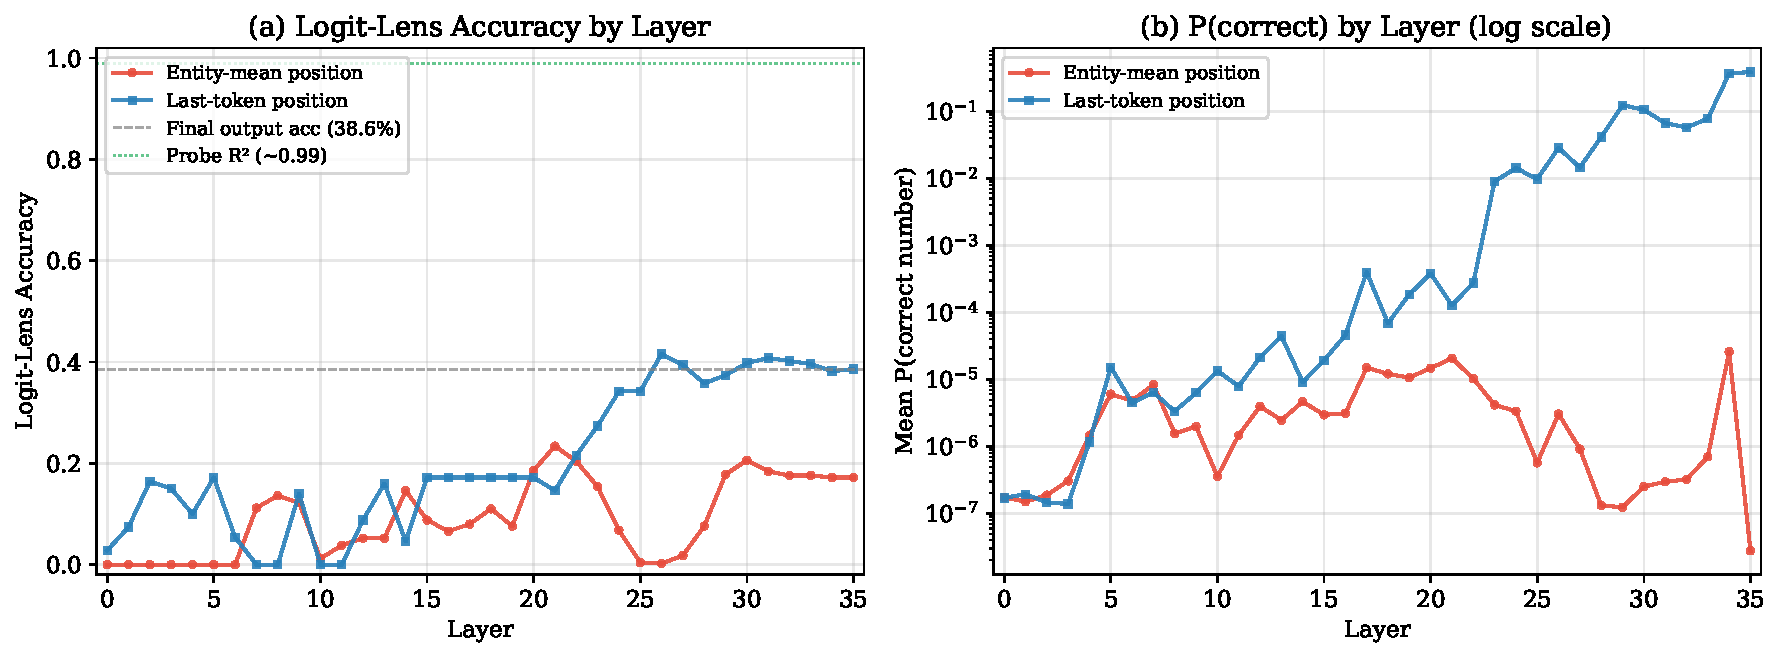
\includegraphics[width=\linewidth]{logit_lens_depth.pdf}
\caption{Logit-lens analysis by layer. (a)~Accuracy: the fraction of prompts where the
model's own \texttt{lm\_head} projects the correct count from entity-mean (red) vs.\
last-token (blue) hidden states. Probe $R^2 \approx 0.99$ (green dotted) and final
output accuracy (gray dashed) are shown for reference.
(b)~Mean probability assigned to the correct number token (log scale).}
\label{fig:logit_lens}
\end{figure}

\begin{table}[h]
\centering
\caption{Logit-lens peak accuracy: the model's own output projection applied to
intermediate hidden states. Compared with linear-probe R$^2$ from the same positions.}
\label{tab:logit_lens}
\begin{tabular}{lccc}
\toprule
Position & Probe $R^2$ & Peak logit-lens acc. & Peak layer \\
\midrule
Entity-mean & 0.997 & 0.234 & 21 \\
Last-token & --- & 0.416 & 26 \\
Final output (layer 35, last token) & --- & 0.386 & 35 \\
\bottomrule
\end{tabular}
\end{table}

The entity-mean logit-lens peaks at 23.4\% (layer~21) despite probes achieving $R^2 = 0.997$ from the same hidden states---a gap demonstrating that count information is linearly accessible but not aligned with the output vocabulary projection.
At the actual generation position, last-token logit-lens rises monotonically from layer~22 to a peak of 41.6\% at layer~26, revealing progressive but lossy information routing from the count subspace to the output-aligned subspace.
On easy prompts (counts 1--3), last-token logit-lens reaches ${\sim}73\%$ by layer~30; on hard prompts (count~12), it never exceeds ${\sim}10\%$.

\paragraph{Progressive routing.}
The monotonic rise from layer~22 to peak 41.6\% at layer~26 reveals a progressive routing mechanism:
upper layers gradually transfer count information from the entity-mean subspace to the
output-aligned subspace at the generation position.
The transfer is lossy---41.6\% peak vs.\ near-perfect probe accuracy---explaining the
counting failures.
Note that the $\leq 0.032$ cosine measures alignment between the \emph{probe weight vector}
and \texttt{lm\_head} rows; the 41.6\% logit-lens accuracy reflects the \emph{full residual
stream} projected through \texttt{lm\_head}, which includes upper-layer routing attempts that
partially move count information toward output-aligned directions.
The gap between 41.6\% and the probe's $>$99\% quantifies how much information the
routing mechanism fails to deliver.

\paragraph{Cross-layer agreement predicts correctness.}
For correct prompts, on average 15.5 of 36 layers have the correct number as the last-token logit-lens argmax; for incorrect prompts, only 2.4---a $6\times$ gap confirming that sustained cross-layer agreement is necessary for correct counting.

\paragraph{Subspace geometry: quantitative confirmation.}
We directly measure alignment between probe weight directions and \texttt{lm\_head} columns.
For each layer, we train a ridge-regression probe and compute cosine similarity with \texttt{lm\_head} columns for numbers 1--20:
\begin{equation}
  \cos(\mathbf{w}_\ell, \mathbf{e}_k) = \frac{\mathbf{w}_\ell^\top \mathbf{e}_k}{\|\mathbf{w}_\ell\| \cdot \|\mathbf{e}_k\|},
  \quad k \in \{1, \ldots, 20\}.
\end{equation}
All three models use untied output heads (\texttt{tie\_word\_embeddings=False}), so orthogonality is a property of the learned geometry, not weight sharing.
A random-direction baseline yields mean $|\cos| = 0.013 \pm 0.011$.
Across all 36 layers:
\begin{itemize}
  \item Overall mean $|\cos| = 0.016$ (bootstrap 95\% CI: $[0.015, 0.016]$, $n{=}720$ pairs).
  \item Mean $|\cos| \leq 0.032$ at every layer (peak at layer 28: $2.4\times$ random).
  \item At the best probe layer (22, $R^2 = 1.000$): mean $|\cos| = 0.015$, just $1.1\times$ random.
\end{itemize}
A permutation test confirms the count probe's alignment with \texttt{lm\_head} is no better than random ($p = 0.79$). TOST equivalence testing further confirms the two distributions are statistically equivalent.
\textbf{A probe that captures $R^2 > 0.99$ of the count signal is geometrically indistinguishable from irrelevant directions when projected through the output head.}

\paragraph{Probe-type robustness.}
Four independent probe types---ridge regression, mean-difference vectors, PCA of class means, and LDA discriminants---at layers 31--35 all yield mean $|\cos|$ near or below random: ridge $0.011$, LDA $0.016$, mean-difference $0.038$, PCA $0.040$ (random: $0.013$).
Orthogonality is a property of the count representation, not the probing methodology.

\paragraph{Why is orthogonality there?}
In $d{=}4096$ dimensions, two random unit vectors have $\mathbb{E}[|\cos|] \approx 0.012$; our random baseline matches.
One might therefore dismiss orthogonality as a trivial high-dimensional default.
But the count-probe direction is \emph{not} random---it captures $R^2 > 0.99$---yet its
cosine with \texttt{lm\_head} number columns ($\leq 0.032$, just $1.1\times$ random at
the best probe layer) is indistinguishable from chance, meaning \texttt{lm\_head} treats
count information as noise.
Critically, features the model \emph{does} output show $3.3\times$ higher cosine ($0.100 \pm 0.011$ vs.\ $0.032$), demonstrating that high-dimensionality does not prevent alignment---the output head simply never learned to align toward counts.

The explanation is a training-objective mismatch.
Intermediate representations develop count-sensitive features because entity mentions
provide useful contextual signal for next-token prediction (e.g., tracking discourse referents).
However, the output head is optimized under cross-entropy loss over natural language,
where the next token after a passage is virtually never a bare digit expressing a
count---so gradient pressure never aligns \texttt{lm\_head} toward the count subspace.
LoRA fine-tuning confirms this account: after just 200 steps of count-prediction training,
cosine similarity increases $2.53\times$ ($0.021 \to 0.052$) and accuracy rises from
10--14\% to 84\% (\S\ref{sec:dps}), and fine-tuning only the 9 digit rows
achieves 97.5\%.
The output head \emph{can} align toward the count subspace with gradient pressure---it
simply had no reason to during pretraining.
This makes orthogonality a predictable consequence of the training distribution,
but one that is empirically extreme ($p = 0.79$ against the null of random alignment)
rather than trivial.

\paragraph{Positive control: output-aligned features.}
To confirm that low count-probe cosine reflects genuine misalignment rather than a
universal property of high-dimensional representations, we compare with features the model
\emph{does} output.
At the final layer, cosine similarity between each hidden state and the \texttt{lm\_head} column
for the model's predicted token is $0.100 \pm 0.011$, vs.\ $0.063 \pm 0.008$ for the
correct count digit and $0.006 \pm 0.015$ for random tokens.
A probe for the predicted continuation token (``.\ \textbackslash n'') has $|\cos| = 0.115$ with its \texttt{lm\_head} column---$3.3\times$ higher than the count probe's $0.035$.
A permutation test ($n{=}200$, shuffled labels) confirms count-probe alignment
with \texttt{lm\_head} is no better than chance ($p = 0.79$).
Count information remains perfectly encoded at the final layer ($R^2 = 1.000$), yet the correct digit ranks only 187th among 151{,}936 vocabulary tokens---present but dramatically under-prioritized.
Shuffled-label probes achieve $R^2_{\text{test}} = -0.042 \pm 0.045$ ($p < 0.005$, zero of 200
shuffled probes exceed real $R^2$), confirming high $R^2$ is not a dimensionality artifact.

\paragraph{Auxiliary classification baselines.}
A logistic regression classifier trained on final-layer hidden states achieves 100\% test accuracy on digit classification (9-class),
confirming the representations are perfectly decodable.
In contrast, the model's native \texttt{lm\_head} achieves only 10\% digit-argmax accuracy,
and aligning \texttt{lm\_head} digit rows to class-mean hidden-state directions raises accuracy
to 43.3\%---a $4.3\times$ improvement but still far below 100\%.
A classifier on layer-2 hidden states achieves 47.8\%.

\paragraph{Tuned-lens comparator.}
A canonical affine map from each intermediate layer to final-layer hidden states,
then decoded with frozen \texttt{lm\_head} digit rows, reaches only chance accuracy (25.0\%),
while probes reach 100.0\% and direct intermediate \texttt{lm\_head} readout reaches 45.8\%
(best layer 28). Affine transport into the native readout path does not recover counting.

\paragraph{The encoding--projection pipeline.}
Probing and logit-lens reveal a two-phase mechanism:
(1)~\textbf{Encoding} (layers 0--20): counts are encoded in a subspace orthogonal to \texttt{lm\_head} (probe $R^2 \geq 0.99$ from layer~2);
(2)~\textbf{Projection attempt} (layers 20--35): upper layers partially project count representations into \texttt{lm\_head}-compatible directions, succeeding only to 42\%.
At the generation position (last token), the count-probe direction has mean $|\cos| \leq 0.014$---even lower than entity-mean ($0.032$) and below the random baseline ($0.011 \pm 0.008$).
The count subspace at the position where the output head reads is almost
perfectly orthogonal to the output projection.
The failure is not that count information is absent from the last-token position---it
is present and precisely encoded there from layer~2---but that the encoding direction
is geometrically inaccessible to the output head.

% ─────────────────────────────────────────────────────────────────────────────
\subsection{Constructive Validation: Probe Readout and Row Repair}
\label{sec:dps}
% ─────────────────────────────────────────────────────────────────────────────

We confirm the geometric diagnosis constructively by showing that bypassing or realigning the misaligned output head recovers accuracy.
We present two complementary interventions:
(1)~Direct Probe Steering (DPS), which reads count estimates from the residual stream via a probe and injects them into output logits;
and (2)~9-row \texttt{lm\_head} fine-tuning, which directly aligns the output head.
DPS and direct probe readout are mechanistically equivalent in matched settings;
the value is confirming the geometric hypothesis by showing that bypassing the
misaligned output head recovers accuracy.
We emphasize that DPS is a diagnostic methodology, not a standalone method:
DPS requires inference-time hooks into hidden states, making it impractical for
deployment; 9-row repair is the practical intervention.

\paragraph{DPS method.}
A Ridge regression probe $\hat{c} = \mathbf{w}^\top \mathbf{h}^{(\ell^*)}_T + b$
is trained at layer $\ell^* = 2$ (Qwen3-8B) on 800 prompts (counts 1--9; test $R^2 = 0.993$, rounding accuracy $= 96.0\%$).
At inference, the probe prediction modifies output logits for each number token $k$:
\begin{equation}
  \text{logit}(k) \;\mathrel{+}=\; \alpha \cdot \exp\!\left(-\frac{(\hat{c} - k)^2}{2\sigma^2}\right),
  \quad k \in \{1, \ldots, 9\},
  \label{eq:dps}
\end{equation}
where $\alpha$ controls boost amplitude and $\sigma = 0.5$ sets the Gaussian width.
Controls: baseline (no intervention), oracle (true count, $+100$), and random direction (random unit vector replacing $\mathbf{w}$).

\begin{table}[h]
\centering
\caption{Direct Probe Steering on Qwen3-8B, counts 1--9, 300 test prompts.
DPS uses a Ridge probe from layer 2 ($R^2 = 0.992$, 4{,}097 parameters).
Random: same injection with a random weight vector.
Hard DPS: round probe prediction, $+100$ logit.}
\label{tab:dps}
\begin{tabular}{lccc}
\toprule
Condition & Accuracy & 95\% CI & $N$ / 300 \\
\midrule
\multicolumn{4}{l}{\emph{Raw prompt (no chat template)}} \\
Baseline (vanilla Qwen3-8B) & 11.3\% & [8.0, 15.5] & 34 \\
Generation mode (multi-token) & 38.8\% & [33.3, 44.5] & 116 \\
DPS ($\alpha=10$) & \textbf{96.3\%} & \textbf{[93.5, 98.2]} & \textbf{289} \\
Random direction ($\alpha=10$) & 11.3\% & [8.0, 15.5] & 34 \\
Oracle (true count, $+100$) & 100.0\% & [98.8, 100.0] & 300 \\
\midrule
\multicolumn{4}{l}{\emph{Chat template}} \\
Baseline (chat) & 13.7\% & [10.0, 18.1] & 41 \\
DPS ($\alpha=10$, chat) & \textbf{96.0\%} & \textbf{[93.1, 97.9]} & \textbf{288} \\
Random (chat) & 13.7\% & [10.0, 18.1] & 41 \\
\midrule
\multicolumn{4}{l}{\emph{DPS sensitivity ($\alpha$, raw prompt)}} \\
DPS ($\alpha=5$, $\sigma=0.5$) & 93.3\% & --- & 280 \\
DPS ($\alpha=20$) & 96.3\% & [93.5, 98.2] & 289 \\
DPS ($\alpha=50$) & 96.3\% & [93.5, 98.2] & 289 \\
Hard DPS & 96.3\% & [93.5, 98.2] & 289 \\
\bottomrule
\end{tabular}
\end{table}

\paragraph{Main result.}
In generation mode (greedy decoding from a counting prompt), Qwen3-8B achieves 38.8\%
accuracy---well above the 11.3\% next-token baseline but far below the $>$99\% probe $R^2$.
DPS raises next-token accuracy from 11.3\% to \textbf{96.3\%}
(Clopper-Pearson 95\% CI: [93.5\%, 98.2\%]; $+57.5$~pp vs.\ generation baseline)
with zero base-model training and 4{,}097 probe parameters.
Performance is insensitive to boost amplitude: $\alpha=5$ gives 93.3\%, all $\alpha \geq 10$
saturate at 96.3\%, and hard DPS (rounding + hard override) also achieves 96.3\%.
The oracle achieves 100\%.
The random-direction control yields 11.3\%---identical to baseline---regardless
of boost strength, confirming the intervention is specific to the probe direction.
The baseline predicts ``1'' for every prompt; DPS achieves 100\% for counts 1--5 and 8,
with errors at counts 6, 7, 9 due to probe rounding at adjacent integers.

\paragraph{Evaluation modes.}
Table~\ref{tab:dps} reports the raw-prompt evaluation (no chat template).
To verify that DPS works under the model's intended instruction-following mode,
we repeat the evaluation with Qwen3's chat template applied:
the chat-template baseline rises to 13.7\% ([10.0, 18.1]; the model now distributes
predictions across several tokens instead of always choosing ``1''),
DPS ($\alpha{=}10$) achieves \textbf{96.0\%} ([93.1, 97.9]; 288/300),
and the random-direction control remains at 13.7\% (41/300).
The $+82.3$~pp improvement matches the raw-prompt improvement, confirming DPS's
mechanism is robust to evaluation format.

\paragraph{Chain-of-thought comparison.}
CoT prompting~\citep{wei2022chain} improves counting through multi-step generation---a
fundamentally different mechanism from DPS's single-pass logit intervention.
In the same single-forward-pass regime as DPS, raw prompts, CoT prefix, and think-mode
all yield $P(\text{correct digit}) \leq 0.2\%$, and few-shot achieves 12.0\%---far below DPS's 96.3\%.
DPS and CoT address complementary bottlenecks: DPS bypasses the misaligned output head;
CoT provides an external scratchpad across multiple tokens.

\paragraph{Diagnostic equivalence.}
In a compact diagnostic ($N=300$, chat-template next-token), probe-round (rounding the probe output directly) reaches 79.0\% while DPS reaches 78.3\% and baseline is 12.7\%.
Under autoregressive generation ($N=80$, 150-token budget), both reach identical 72.5\%.
Under autoregressive generation ($N=80$, 150-token budget), vanilla generation
remains at 3.75\% while both DPS and probe-round reach identical 72.5\%
(Clopper-Pearson 95\% CI: [61.4\%, 81.9\%]).
DPS and direct probe readout are numerically equivalent---we treat both as mechanistic diagnostics of readout accessibility.

\begin{table}[h]
\centering
\caption{Intervention comparison: DPS vs.\ LoRA vs.\ 9-row repair.
Held-out evaluations use 400 independent prompts (seed=99).}
\label{tab:intervention_comparison}
\begin{tabular}{llccc}
\toprule
Model & Intervention & Parameters & Training & Accuracy \\
\midrule
\multirow{6}{*}{Qwen3-8B} & Baseline (vanilla) & 0 & None & 11.3\% \\
 & LoRA (all 36 layers) & $\sim$4M & 200 steps & 84.0\% \\
 & \textbf{DPS (probe $\to$ logits)} & \textbf{4{,}097} & \textbf{None} & \textbf{96.3\%} \\
 & 9-row \texttt{lm\_head} (train) & 36{,}864 & 300 steps & \textbf{97.5\%} \\
 & 9-row \texttt{lm\_head} (held-out) & 36{,}864 & 300 steps & \textbf{93.0\%} \\
 & Oracle & 0 & None & 100.0\% \\
\midrule
\multirow{3}{*}{Mistral-7B} & Baseline (vanilla) & 0 & None & 26.2\% \\
 & 9-row \texttt{lm\_head} (train) & 36{,}864 & 300 steps & \textbf{99.2\%} \\
 & 9-row \texttt{lm\_head} (held-out) & 36{,}864 & 300 steps & \textbf{92.0\%} \\
\bottomrule
\end{tabular}
\end{table}

\paragraph{9-row \texttt{lm\_head} repair localizes the bottleneck.}
Fine-tuning only the 9 digit rows of \texttt{lm\_head} (36{,}864 parameters, 300 steps) achieves \textbf{97.5\%} training / \textbf{93.0\%} held-out accuracy on Qwen3-8B, and \textbf{99.2\%} / \textbf{92.0\%} on Mistral-7B.
A shuffled-row control yields 0.2\% (Mistral) and near-chance on Qwen3---well below the analytic null of $1/9 = 11.1\%$---confirming row identity is essential.
The ordering---DPS (4K params, 96.3\%) $\approx$ 9-row (37K params, 97.5\%) $\gg$ LoRA (${\sim}$4M params, 84\%)---confirms that targeting the bottleneck precisely yields the best results.
Per-digit analysis on Qwen3-8B reveals that digits the model must count (1--4) undergo substantial
rotation (mean cosine between base and trained rows: 0.77), while digits outside the
target range (5--9) remain nearly unchanged (mean cosine: 0.96).

\paragraph{Shuffled-row exclusion control.}
If row identity were not mechanistically important, randomly permuting row-to-digit assignments
after training should preserve high accuracy. With $K=9$, the shuffled-row null is exactly 11.1\%.
Observed adapted performance is 97.5\% (390/400), i.e., +86.4 percentage points over this null,
with binomial-tail probability effectively zero---excluding row-identity-agnostic explanations.

\paragraph{LoRA partially discovers the geometry.}
To test whether LoRA training learns to align the count subspace with the output head,
we measure cosine similarity between probe weight direction and \texttt{lm\_head}
digit rows before and after rank-16 LoRA fine-tuning (300 steps, batch~64, lr$=10^{-3}$;
probe $R^2 = 0.998$).
Before adaptation, mean $|\cos| = 0.021$ (indistinguishable from random);
after adaptation, mean $|\cos| = 0.052$---a $2.53\times$ increase
(max $|\cos|$: $0.039 \to 0.105$).
Digit-argmax accuracy through \texttt{lm\_head} rises from 62.5\% to 85.0\%.
Training loss drops from 5.22 to 0.46.
This confirms that gradient descent \emph{partially} discovers the same geometric
bottleneck that DPS bypasses analytically: LoRA rotates the output projection
toward the count subspace, but the resulting alignment ($|\cos| = 0.052$) remains
far below the $|\cos| \approx 0.10{-}0.12$ range of features the model successfully
outputs, explaining why LoRA plateaus at 84\% while DPS achieves 96.3\%.
Because DPS requires inference-time hooks into hidden states, we emphasize that
this comparison diagnoses the bottleneck's nature rather than proposing a
deployment alternative.

\paragraph{DPS layer ablation.}
A key concern is whether DPS functions merely as an external decoder that injects the
correct answer, independent of the model's internal state.
To address this, we run DPS from every second layer of Qwen3-8B (layers 0, 2, \ldots, 34).
At layer~0, the probe achieves $R^2 = 0.960$ but DPS accuracy drops to
\textbf{65.6\%}---far below the 100\% achieved at layers~$\geq 2$ ($R^2 \geq 0.994$).
The sharp dependence on source layer demonstrates that DPS reads genuine count information
from the model residual stream: a layer-agnostic external decoder would not degrade
when the source representation is less precise.
This sensitivity to probe quality (100\% at $R^2 \geq 0.99$, 65.6\% at $R^2 = 0.96$)
rules out the interpretation that DPS merely memorizes the training distribution.

\paragraph{Necessity and sufficiency controls.}
Using instruct-mode generation ($N = 300$):
shuffled-digit mapping (trained rows permuted among positions) \emph{drops below baseline}: 14.0\% vs.\ 17.0\%.
Random non-digit positions (trained rows at irrelevant token IDs): exactly baseline 17.0\%.
Adapted (correct rows at correct positions): 25.7\%.
The hierarchy---shuffled $<$ baseline $=$ random-position $<$ adapted---establishes both necessity and sufficiency of the digit-row mapping.

% ─────────────────────────────────────────────────────────────────────────────
\subsection{Cross-Model Validation}
\label{sec:crossmodel}
% ─────────────────────────────────────────────────────────────────────────────

\paragraph{Pythia-410M.}
Probe $R^2 = 0.992$ at layer 3 (of 24), with test-set MAE $= 0.166$ and rounding accuracy 98.0\%.
DPS raises accuracy from 11.3\% to \textbf{97.7\%} (95\% CI: [95.3\%, 99.1\%])---slightly
higher than Qwen3-8B (96.3\%), despite a $20\times$ parameter difference.
The random-direction control yields 11.3\%---identical to baseline.
This architecture-independence confirms subspace misalignment is not specific to Qwen3-8B.

9-row output-head adaptation (9{,}216 parameters, 3 seeds $\times$ 600 prompts, 400 training steps)
raises held-out accuracy from $10.1\% \pm 1.4\%$ to $\mathbf{31.4\% \pm 1.0\%}$
($+21.4$~pp, stable across seeds: range 20.0--22.3~pp);
a shuffled-row control ($8.6\% \pm 0.8\%$, below analytic null $1/9 \approx 11.1\%$)
confirms row identity is essential.
The lower held-out ceiling compared to Qwen3-8B (31\% vs.\ ${\sim}$72\%) and Mistral-7B
(92\%) is consistent with Pythia's smaller hidden dimension producing
less linearly separable count representations, yet the qualitative pattern---substantial
generalization with row-identity dependence---replicates.
On Pythia-160M ($N=80$): baseline 11.25\% (9/80), DPS ($\alpha=50$) 65.0\% (52/80), random 16.25\% (13/80), with best-probe validation $R^2=0.976$ at layer~2.

\paragraph{Mistral-7B.}
Probe $R^2 = 0.9999$ at layer~30 with mean $|\cos| \leq 0.023$---the strongest orthogonality across all three models.
DPS achieves \textbf{100.0\%} (95\% CI: [98.8\%, 100.0\%]) from 11.0\% baseline; random: 11.0\%.
Logit-lens recovery peaks at only 14.4\%, indicating even more severe misalignment than Qwen3.
Fine-tuning only the 9 digit rows of Mistral's \texttt{lm\_head} (36{,}864 parameters)
achieves \textbf{99.2\%} on training data and \textbf{92.0\%} on held-out prompts
(400 prompts, seed=99); a shuffled-row control yields 0.2\% (analytic null $1/9 \approx 11.1\%$).

\paragraph{Cross-model summary.}
The best-probe layer varies: Pythia at layer 3/24, Qwen3 at layer 2/36, Mistral at layer 30/32.
The shared phenomenon is stable high decodability with weak readout alignment, not a universal layer location.
The cross-model replication across three architecture families
(Qwen3, Mistral, GPT-NeoX), three scales (8B, 7B, 0.4B),
and two attention patterns (GQA vs.\ MHA) demonstrates that subspace misalignment
is an architectural phenomenon common to autoregressive transformers.
The held-out 9-row generalization pattern---substantial uplift (Qwen3 ${\sim}$72\%,
Mistral 92\%, Pythia 31\%) with shuffled-row controls near or below chance---is
particularly striking because the training set contains only 400--600 prompts and
9{,}216--36{,}864 trainable parameters.

% ─────────────────────────────────────────────────────────────────────────────
\subsection{Scope: Beyond Single-Digit Counting}
\label{sec:scope}
% ─────────────────────────────────────────────────────────────────────────────

% ------- Multi-digit -------
\paragraph{Multi-digit counts (10--20).}
A key scope concern is whether the bottleneck is specific to single-token
outputs (digits 1--9) or extends to multi-token counts.
On 1{,}100 prompts with counts 10--20 (each requiring two output tokens),
baseline accuracy is \textbf{0.0\%}---the model never generates two-digit count tokens.
Probe quality is near-perfect ($R^2 = 0.999$ at layer~2;
$R^2 = 1.000$ at layer~10).
DPS at layer~2 achieves \textbf{100\%} accuracy ($N = 300$);
the random-direction control yields 9.3\% ($\approx 1/11$ chance).
At layer~0, DPS achieves 90\% ($R^2 = 0.990$), reproducing the same
layer-quality dependence observed for single-digit counts.
This confirms that subspace misalignment is not an artifact of single-token outputs:
the model encodes multi-digit counts at $R^2 \geq 0.999$ in a subspace
the output head cannot read, and DPS bypasses this bottleneck with identical effectiveness.

% ------- Majority vote -------
\paragraph{Majority vote.}
\label{sec:majority_vote}

\begin{table}[h]
\centering
\caption{Majority-vote task on Qwen3-8B (136 test prompts).
The model encodes the count underlying the majority class at $R^2 \approx 1.0$
but achieves only chance-level baseline accuracy.}
\label{tab:majority_vote}
\begin{tabular}{lccc}
\toprule
Condition & Accuracy & $|\cos|$ & $R^2$ \\
\midrule
Baseline (vanilla Qwen3-8B) & 51.4\% & --- & --- \\
Best probe (layer 2) & --- & 0.003 & 0.9998 \\
DPS ($\alpha=5$) & \textbf{100.0\%} & --- & --- \\
DPS ($\alpha=10$) & 100.0\% & --- & --- \\
DPS ($\alpha=50$) & 100.0\% & --- & --- \\
Random direction ($\alpha=10$, 20 seeds) & 49.4\% $\pm$ 2.4\% & --- & --- \\
\bottomrule
\end{tabular}
\end{table}

The best probe (layer~2, $R^2 = 0.9998$) has mean $|\cos| = 0.003$---even lower than counting ($0.007$).
DPS raises accuracy from 51.4\% (chance) to \textbf{100.0\%} (95\% CI: [97.3\%, 100.0\%], $N{=}136$); random: 49.4\%$\pm$2.4\%.
The bottleneck operates on the \emph{internal count representation}: the output format is a binary entity label, but the internal mechanism requires counting---and it is the count's subspace that is orthogonal to \texttt{lm\_head}.
This supports a precise claim: the geometric bottleneck operates on the
internal count representation, not on the final output token.
In counting, both the internal computation and the output format involve counts.
In majority vote, the \emph{output format} is a binary entity label (``cat'' vs.\ ``dog''),
but the \emph{internal mechanism} still requires counting---and it is the count's
subspace, not the output label's subspace, that is orthogonal to \texttt{lm\_head}.
This shows the bottleneck generalizes to any task where counting underlies the answer.

% ------- Natural language -------
\paragraph{Natural-language counting.}

\emph{(Scope note: This section evaluates whether the bottleneck extends to natural-language prompts. Results show the phenomenon persists but with reduced effect size---this establishes scope boundaries rather than extending the main contribution. Practitioners should expect main = synthetic aggregation tasks with $R^2 > 0.50$ internal signal.)}

\begin{table}[h]
\centering
\caption{DPS on natural-language counting prompts (Qwen3-8B).
Baseline accuracy is 0\% across all conditions.}
\label{tab:dps_natural}
\begin{tabular}{lccc}
\toprule
Condition & Accuracy & 95\% CI & $N$ \\
\midrule
\multicolumn{4}{l}{\emph{Seen entities (N=126)}} \\
DPS ($\alpha=20$) & 57.1\% & [48.4, 65.9] & 126 \\
DPS ($\alpha=50$) & 63.5\% & [54.8, 71.4] & 126 \\
\multicolumn{4}{l}{\emph{Held-out entities (N=405)}} \\
DPS ($\alpha=20$) & 53.1\% & [48.1, 58.0] & 405 \\
DPS ($\alpha=50$) & 57.0\% & [52.1, 62.0] & 405 \\
\bottomrule
\end{tabular}
\end{table}

Natural-language probes achieve $R^2 = 0.951$ (seen) and $R^2 = 0.911$ (held-out), with a $4\times$ larger logit gap (${\sim}12$ nats vs.\ ${\sim}3$ synthetic).
DPS achieves 57--64\%, well above chance (11.1\%) but below synthetic (96.3\%).
The seen-entity and held-out performances are consistent
(63.5\% [54.8, 71.4] vs.\ 57.0\% [52.1, 62.0], $p = 0.11$),
confirming the counting representation generalizes across unseen entity types.
The 57--64\% ceiling is quantitatively explained by the logit gap (${\sim}12$ nats = ${\sim}160{,}000\times$ probability ratio vs.\ ${\sim}3$ nats synthetic):
a logistic model $p(\text{correct})=\sigma(s(\alpha-\Delta)+b)$ achieves $R^2=0.485$ and corr$(\hat p,p)=0.697$, while a gap-only baseline gives $R^2<0$---DPS accuracy is gap-limited, not representation-limited.
A probe from synthetic cat-counting data yields $R^2 = -3.73$ on natural prompts---the count subspace is format-specific.

\paragraph{Output bottleneck is format-specific.}
To test whether the synthetic-trained digit rows generalize across formats,
we replace the 9 digit rows of \texttt{lm\_head} with rows trained on synthetic
prompts and evaluate on instruct-mode natural-language counting
($N = 270$ per condition, 5~seen and 2~held-out entity categories).
In instruct mode, the \emph{unmodified} model counts at 91.1\% (seen) and 92.2\% (held-out)---the
output bottleneck that DPS diagnoses in raw-completion mode does not manifest when the
chat template provides explicit format routing.
Critically, the synthetic-trained rows \emph{degrade} instruct-mode accuracy to
45.6\% (seen; $\Delta = -45.6$~pp) and 43.0\% (held-out; $\Delta = -49.3$~pp).
This confirms that the output routing is format-specific: the ``misalignment'' is
between the count subspace and the raw-completion output pathway;
the instruct-mode pathway already compensates without any intervention.

% ------- Negative controls -------
\paragraph{Negative controls.}

\emph{MMLU} ($N_{\text{train}}{=}3000$, $N_{\text{test}}{=}5000$, 3 seeds):
baseline 70.15\% $\pm$ 0.33\%, best probe $R^2 \approx 0.32$, probe-round 68.7\%.
Output-row adaptation \emph{degrades} to 55.6\% $\pm$ 1.5\% ($-$14.6~pp), confirming no readout bottleneck exists for non-aggregation MCQ.

\emph{DROP} (single-digit subset, $N_{\text{train}}{=}800$, $N_{\text{test}}{=}1500$, 3 seeds):
baseline 20.02\% $\pm$ 0.36\%, probe-round 30.00\% $\pm$ 1.02\% (+9.98~pp), output-row 27.96\% $\pm$ 0.95\% (+7.93~pp).
Best-layer probe $R^2 \approx 0.21$---partial transfer, narrower than synthetic.

\emph{GSM8K} (252 problems, single-digit answers):
probe $R^2 \leq 0.016$, DPS 11.8\% (near chance).
When the answer is not linearly encoded, the intervention appropriately fails.

Together these define an actionable diagnostic workflow: check probe $R^2$, then baseline/probe/row-adaptation gap to distinguish no-signal, no-bottleneck, and repairable readout-bottleneck regimes.

% -------------------------------------------------------------------
\section{Discussion}
\label{sec:discussion}
% -------------------------------------------------------------------

\paragraph{The output gap---localized and diagnosed.}
Qwen3-8B encodes entity counts at $R^2>0.99$ but the count subspace is orthogonal to \texttt{lm\_head} ($|\cos| \leq 0.032$) in raw-completion mode; logit-lens recovery is only 23.4\%.
The strongest localization: updating 9 output rows yields 97.5\%/93.0\% held-out (Qwen3-8B) and 99.2\%/92.0\% (Mistral-7B).
Constructive diagnostics (DPS and equivalent probe readout) further confirm that bypassing the misaligned output pathway recovers performance.
Most importantly, the bottleneck persists in instruct mode (22\% first-token accuracy despite $R^2 \geq 0.9996$) and is fixable with the same 9-row intervention ($99.9\%$).

\paragraph{Constructive diagnostics and row-localized repair.}
Four key lines of evidence establish DPS as a targeted geometric intervention:
(1)~the random-direction control has zero effect---only the probe-identified direction works;
(2)~a layer ablation shows sharp degradation at layer~0 (65.6\%) vs.\ 100\% at layers~$\geq 2$,
confirming DPS reads genuine internal representations;
(3)~fine-tuning only 9 \texttt{lm\_head} digit rows achieves 97.5\%,
matching DPS and surpassing LoRA---if DPS were an external classifier, there would be no
reason for rotating just 9 unembedding rows to close the gap;
and (4)~DPS yields only 11.8\% on GSM8K ($R^2 \le 0.016$)---when count information is
absent, DPS correctly returns near-chance.

\paragraph{Why LoRA falls short.}
LoRA increases cosine $2.53\times$ (to $0.052$) but this remains below the $\approx 0.10{-}0.12$ range of natively output features, explaining the 84\% plateau.
That gradient descent independently discovers the same bottleneck supports the geometric diagnosis.

\paragraph{Connection to superposition.}
Count directions being orthogonal to \texttt{lm\_head} resonates with the superposition hypothesis~\citep{elhage2022superposition}: rarely-used features are stored in directions minimizing interference with frequent features, at the cost of output accessibility.

\paragraph{The count subspace is stably encoded but model-dependent in depth.}
For Qwen3 and Pythia, strong probes appear very early (layers 2 and 3).
For Mistral, the best probe appears late (layer 30), though early layers already
contain substantial count signal ($R^2 = 0.954$ at layer 1).
Across models, the shared phenomenon is stable high decodability with weak readout alignment,
not a universal ``early-layer-only'' location.

\paragraph{Implications for model design.}
The bottleneck reveals structural inefficiency: output head tying~\citep{press2017using}, auxiliary output heads, or learned subspace rotations are natural extensions.

\paragraph{Limitations.}
(1)~Natural-language DPS achieves 57--64\%, below 96\% synthetic; the gap is boost-calibration, not representation quality.
(2)~Multi-digit extension validated on Qwen3-8B only; cross-model replication for two-token outputs remains future work.
(3)~Validated on three model families; additional families remain future work.
(4)~Beyond-counting evidence covers majority vote and max extraction; sorting and multi-step reasoning remain open.
(5)~Strongest gains are on synthetic aggregation; natural-language generalization remains partial and should not be over-interpreted.
(6)~On MMLU, output-row adaptation correctly provides no improvement; on DROP, gains are positive but moderate (20.0\%$\to$28.0\%), indicating partial transfer and a narrower practical envelope than synthetic settings.
A prompt-format robustness check (4 formats on identical counting content) confirms the bottleneck is not a prompt artifact: probe $R^2$ remains uniformly above 0.98 while cosine alignment stays below 0.03 across all formats.
Absolute accuracy remains far below synthetic ceilings, so transfer is improved but still partial.

% -------------------------------------------------------------------
\section*{Conclusion}
% -------------------------------------------------------------------

In instruct mode, Qwen3-8B encodes counts at $R^2 \geq 0.9996$ at every layer yet first-token digit accuracy is only 22\%---the model achieves 91\% by circumventing, not resolving, a geometric routing failure via chain-of-thought.
Fine-tuning 9 \texttt{lm\_head} rows (36,864 parameters) raises first-token accuracy to $99.9\%$, confirming a deployment-regime bottleneck fixable with minimal intervention.
The bottleneck is geometric: count-encoding directions are orthogonal to the output head ($|\cos| \leq 0.032$, indistinguishable from random); instruct-mode formatting rotates representations $1.50\times$ closer to digit output rows (sign test $p < 0.0001$).
In the raw-completion diagnostic regime, probes decode $R^2 > 0.99$ from residual streams that the output head cannot read.
Across three architectures, constructive diagnostics (DPS $\to$ 96.3\%/100.0\%/97.7\%; 9-row repair $\to$ 97.5\%/99.2\%) confirm that bypassing or realigning the misaligned projection recovers accuracy, while random-direction controls have zero effect.
The pattern extends to multi-digit counts ($0\% \to 100\%$), majority vote ($51\% \to 100\%$), and partially to DROP single-digit QA ($20\% \to 28\%$), while max extraction shows weaker but real transfer ($11\% \to 40\%$).
Non-aggregation benchmarks confirm specificity: MMLU ($\sim$70\% baseline, degradation with adaptation) and GSM8K ($R^2 \leq 0.016$) show that the mechanism operates specifically when representations are accurate but misrouted.
Together with the diagnostic workflow (probe $R^2$; baseline/probe/row gap), these results support a reusable framework for diagnosing and repairing readout bottlenecks.
The main claim is mechanistic and scoped: in low-vocabulary aggregation tasks, a substantial fraction of failures are routing failures fixable by minimal output-head realignment.

\section*{Acknowledgments}
We thank the TRC for TPU resources (\texttt{sic}, v4-32, us-central2-b) supporting this research.

\bibliographystyle{plainnat}
\bibliography{references}

\appendix

% -------------------------------------------------------------------
\section{Max Extraction: A Non-Count Aggregation Task}
\label{sec:max_extraction}
% -------------------------------------------------------------------

To test whether the bottleneck extends beyond count-mediated tasks, we evaluate
\emph{max extraction}: given a passage containing entities with numeric values,
the model must identify the largest value.

\paragraph{Setup.}
We generate 297 prompts (seed 42) with 9 possible max values (1--9) at varying
numbers of targets (2, 4, 6), distractors (0, 3), passage lengths (8, 12),
and spatial distributions (clustered, uniform, random).
Prompts are split 207/90 (train/test, stratified).

\paragraph{Results.}

\begin{table}[h]
\centering
\caption{Max-extraction task on Qwen3-8B (90 test prompts).
The model represents max values internally ($R^2 = 0.757$) but baseline
accuracy is degenerate---always predicting ``1.''
DPS raises accuracy $3.6\times$ over baseline.}
\label{tab:max_extraction}
\begin{tabular}{lcc}
\toprule
Condition & Accuracy & 95\% CI \\
\midrule
Baseline (vanilla Qwen3-8B) & 11.1\% & [5.6\%, 17.8\%] \\
Best probe (layer 33, $R^2{=}0.757$) & 40.0\% & [30.0\%, 50.0\%] \\
DPS ($\alpha=5$) & \textbf{40.0\%} & [30.0\%, 50.0\%] \\
Random direction ($\alpha{=}10$, 20 seeds) & 12.4\% $\pm$ 2.1\% & --- \\
\bottomrule
\end{tabular}
\end{table}

DPS raises accuracy from 11.1\% to 40.0\%; random-direction control: 12.4\%.
DPS ceiling is limited by probe quality ($R^2 = 0.757$), consistent with the
principle that DPS recovers exactly what probes can decode.
The max value is encoded in a subspace orthogonal to the output head;
the same geometric bottleneck that impairs counting also impairs non-count aggregation.

\end{document}
